\documentclass{article}

\usepackage{geometry}
\usepackage{makecell}
\usepackage{array}
\usepackage{multicol}
\usepackage{multirow}
\usepackage[table]{xcolor}
\usepackage{setspace}
\usepackage{pdflscape}
\usepackage{changepage}
\usepackage{booktabs}
\usepackage[explicit]{titlesec}
\usepackage{hyperref}
\usepackage{graphicx}
\usepackage{cprotect}
\usepackage{float}
\newcolumntype{?}{!{\vrule width 1pt}}
\newcommand{\paragraphlb}[1]{\paragraph{#1}\mbox{}\\}
\renewcommand{\contentsname}{Inhaltsverzeichnis:}
\renewcommand\theadalign{tl}
\setstretch{1.10}
\setlength{\parindent}{0pt}

\titleformat{\section}
  {\normalfont\Large\bfseries}{\thesection}{1em}{\hyperlink{sec-\thesection}{#1}
\addtocontents{toc}{\protect\hypertarget{sec-\thesection}{}}}
\titleformat{name=\section,numberless}
  {\normalfont\Large\bfseries}{}{0pt}{#1}

\titleformat{\subsection}
  {\normalfont\large\bfseries}{\thesubsection}{1em}{\hyperlink{subsec-\thesubsection}{#1}
\addtocontents{toc}{\protect\hypertarget{subsec-\thesubsection}{}}}
\titleformat{name=\subsection,numberless}
  {\normalfont\large\bfseries}{\thesubsection}{0pt}{#1}

\hypersetup{
    colorlinks,
    citecolor=black,
    filecolor=black,
    linkcolor=black,
    urlcolor=black
}

\geometry{top=12mm, left=1cm, right=2cm}
\title{\vspace{-1cm}Projektmanagement - Projekt}
\author{Andreas Hofer, Samuel Ulz, Patrick Pramberger}

\begin{document}
	\maketitle
	\tableofcontents
	\section{System Design}
	\subsection{Unternehmensbeschreibung}
	Das Bauunternehmen Porr AG hat eine Vielzahl an Standorten und ist europaweit vertreten.
	\subsubsection{Ausgangssituation}
	Um klimaneutraler und umweltfreundlicher zu werden, sollen Kleintransporter der Flotte zu E-Autos getauscht werden. Dabei sollen die Kosten des Betriebs möglichst gleich bleiben.
	\subsubsection{Problemstellung}
	Durch die Vielzahl an Angeboten am Markt ist es unklar, welches Modell die besten Ergebnisse liefert.
	\subsubsection{Vorgehensziel}
	Der Kleintransporter mit dem besten Kosten/Nutzen Verhältnis soll gewählt werden um die klimaneutrale Strategie des Unternehmens umzusetzen.
	\newpage
	\thispagestyle{empty}
	\begin{landscape}
	\subsection{Situationsanalyse}
	\subsubsection{SWOT-Analyse}
	\begin{tabular}{| l | c | c | c | c | c | c | c | c |}
		\toprule
		\multirow{2}*{\makecell{Umwelt\\entwicklung...}} & \multicolumn{4}{| c |}{\makecell{...trifft im System auf eine \\  Stärke oder Schwäche...}} & \multicolumn{3}{| c |}{\makecell{...das bedeutet \\ Chance oder Gefahr}} & ...daher streben wir an...\\ \cline{2-9}
		& + & - & Stärke/Schwäche & Ursachen & + & - & Chance/Gefahr & Erste Ziele \\ \midrule
		\makecell{Umweltförderungen \\ werden \\ verringert/eingestellt} &  &\cellcolor{red!25} x & \makecell{Weniger Geld \\ als Mitbewerber} & \makecell{Geringerer \\ Umsatz} & & \cellcolor{red!25} x & Weniger Budget & Förderungen schnell abrufen \\ \hline

		\makecell{E-Autos werden billiger} & \cellcolor{green!25} x & & \makecell{TODO} & \makecell{TODO} & \cellcolor{green!25}x &  & \makecell{Geringere \\ Anschaffungskosten} & \makecell{Guten  \\Kaufzeitpunkt finden} \\ \hline

		\makecell{Mitarbeiter wollen \\ umweltfreundlichere \\ Autos} & \cellcolor{green!25}x & & \makecell{Unternehmens-\\strategie} & \makecell{Firmenstrategie \\ unterstützt \\ Entwicklung} & \cellcolor{green!25}x & & \makecell{Attraktiverer \\ Arbeitgeber} & \makecell{E-Autos als \\ benefit etablieren} \\ \hline

		\makecell{Wenig \\ ausgeprägte \\ Ladeinfrastruktur} & \cellcolor{green!25}x & & \makecell{Möglichkeit \\ eigene \\ Infrastruktur anzubieten} & \makecell{Viele Bau- und \\ Zweigstellen} & \cellcolor{green!25}x & & \makecell{Selbst \\ Infrastruktur \\ bereitstellen} & \makecell{Bei neuen \\ Baustellen mobile \\ Ladepunkte bereitstellen} \\ \hline
		\bottomrule
	\end{tabular}
	\end{landscape}
	\subsection{Zielformulierung}
	\subsubsection{MUSS-Ziele}
	\begin{enumerate}
		\item{Umwelt und Nachhaltigkeit}
		\begin{itemize}
			\item{$CO_2$-Emissionen des PKW Fuhrparks sollen bis Ende 2027 um mindestens 60\% reduziert werden.}
		\end{itemize}
		\item{Einsatzfähigkeit}
		\begin{itemize}
			\item{Die Mobilität der Mitarbeiter unterschreitet nach dieser Umstellung nicht 95\% des Wertes vor der Umstellung.}
		\end{itemize}
		\item{Ladeverfügbarkeit}
		\begin{itemize}
			\item{Lademöglichkeiten für PKWs an Baustellen und Zweigstellen sollen bis Ende 2027 an 90\% aller Standorte verfügbar sein.}
		\end{itemize}
	\end{enumerate}
	\subsubsection{WUNSCH-Ziele}
	\begin{enumerate}
		\item{Mitarbeiterakzeptanz}
		\begin{itemize}
			\item{Die Zufriedenheit der Nutzer soll innerhalb von 12 Monaten eine positive Feedbackrate von 80\% erreichen}
		\end{itemize}
		\item{Image}
		\begin{itemize}
			\item{Die Umstellung soll bis Ende 2027 zu einer messbaren Verbesserung des Firmenimages führen. Das soll durch Umfragen überprüft werden.}
		\end{itemize}
	\end{enumerate}
	\subsection{Synthese/Analyse}

	\subsection{Bewertung}
	\subsubsection{Paarvergleich}
	\begin{figure}[H]
	\centering
	
\includegraphics[scale=0.35]{images/paarvergleich.png}
	\caption{Paarvergleich}
	\end{figure}
	\begin{figure}[H]
	\centering
	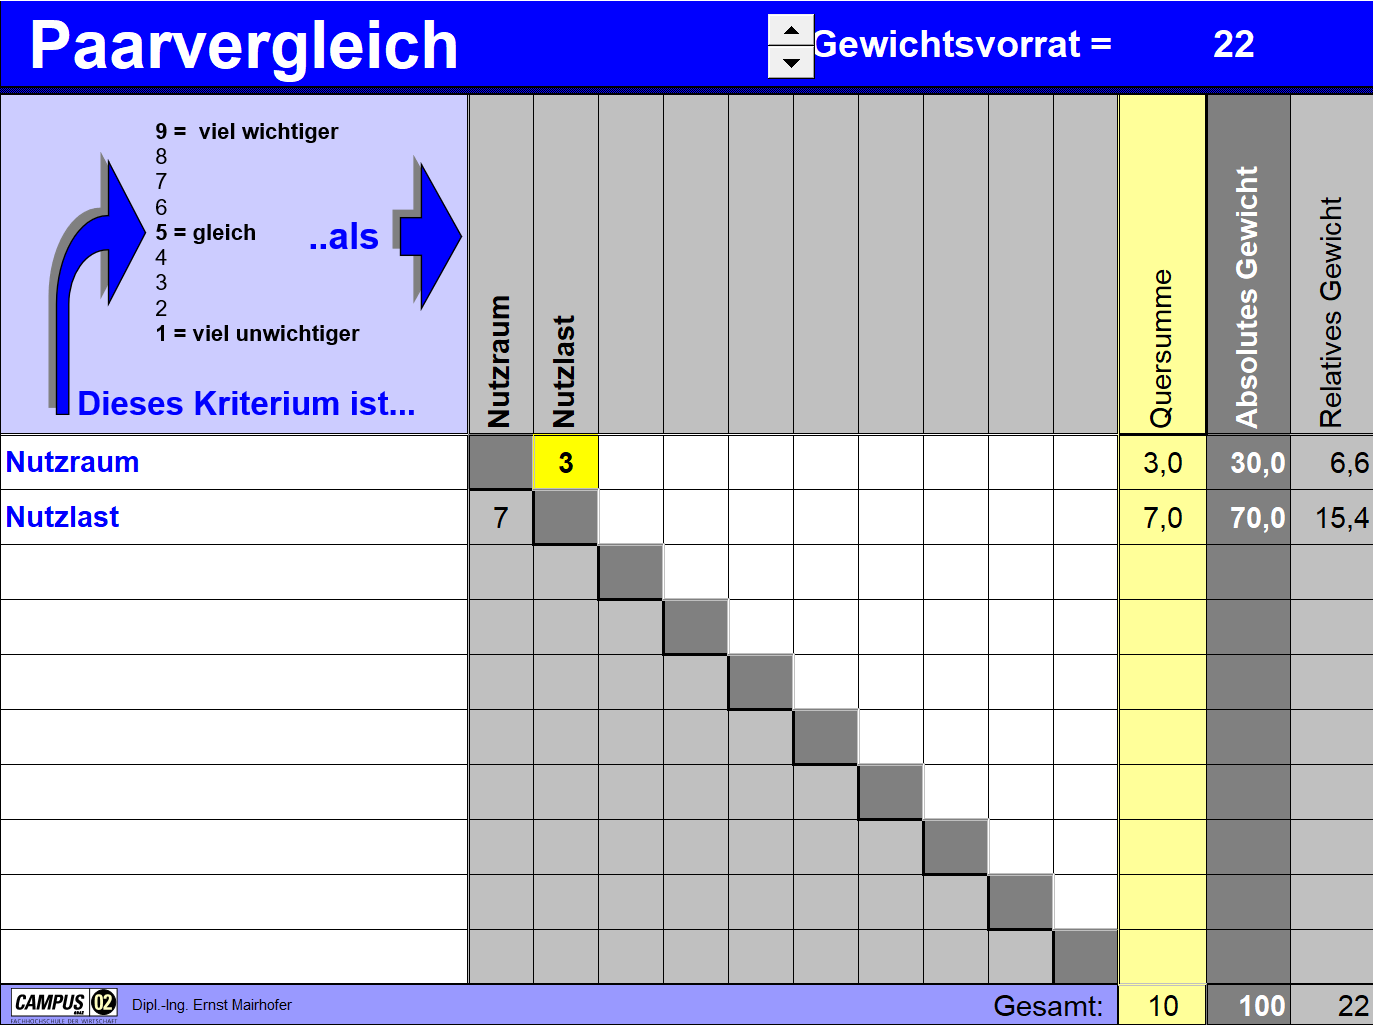
\includegraphics[scale=0.35]{images/paarvergleich2.png}
	\caption{Paarvergleich Nutzraum}
	\end{figure}
	\subsubsection{Daten der Kriterien}
	\begin{tabular}{| c | c | c | c | c | c | c | c |}
		\toprule
		Modell & Preis (€) & \makecell{Motorleistung \\ (kW)} & \makecell{Batterie \\(kWh)} & \makecell{Reichweite \\(km)} &  \makecell{Ladeleistung \\(kW AC/DC)} & \makecell{Nutzfläche \\($m^3$)} & \makecell{Nutzgewicht \\ (kg)}  \\ \midrule
		Ford E-Transit & 49.100 & 160 & 64 & 373 & 11/125 & 6,8 & 994 \\ \hline
		VW ID. Buzz & 54.655 & 210 & 86 & 440 & 11/200 & 3,9 & 744\\ \hline
		Mercedes-Benz eVito & 44.632 & 150 & 90 & 480 & 11/110 & 6,6 & 830\\ \bottomrule
	\end{tabular}
	\subsubsection{Verteilung der Bewertung (Endogen)}
	\begin{tabular}{| l | c | c | c | c | c | c |}
		\toprule
		Modell & \makecell{Motorleistung \\ (kW)} & \makecell{Batterie \\(kWh)} & \makecell{Reichweite \\(km)} &  \makecell{Ladeleistung \\(kW AC/DC)} & \makecell{Nutzfläche \\($m^3$)} & \makecell{Nutzgewicht \\ (kg)}  \\ \midrule
		Ford E-Transit & 1,7 & 0 & 0 & 2 & 10 & 10 \\ \hline
		VW ID. Buzz & 10 & 8,5 & 6,3 & 10 & 0 & 0 \\ \hline
		Mercedes-Benz eVito & 0 & 10 & 10 & 0 & 9,3 & 3,4 \\ \bottomrule
	\end{tabular}
	\subsubsection{Berechnung des Nutzwerts}
	\begin{tabular}{| r  l  l | c | c | c | c | c | c | c | c | }
	\toprule
		\multicolumn{3}{|c|}{\multirow{3}{*}{\textbf{Bewertungskriterien}}} & \multicolumn{2}{|c|}{\multirow{3}{*}{\makecell{Gewicht \\ (G) \\ $\Sigma$ = 100}}} & \multicolumn{6}{| c |}{\textbf{Lösungsvarianten}}  \\ \cline{6-11}
		\multicolumn{3}{|c|}{}&\multicolumn{2}{|c|}{}& \multicolumn{2}{|c|}{\makecell{Ford \\ E-Transit}} & \multicolumn{2}{|c|}{\makecell{VW \\ ID. Buzz}} & \multicolumn{2}{|c|}{\makecell{Mercedes-Benz \\ eVito}} \\ \cline{6-11}
		\multicolumn{3}{|c|}{}&\multicolumn{2}{|c|}{} & B & BxG & B & BxG & B & BxG \\ \hline
		1. && Motorleistung & 9 && 1,6 & 15,3 & 10 & 90 & 0 & 0 \\ \hline
		2. && Batterie & 23 && 0 & 0 & 8,5 & 195,5 & 10 & 230 \\ \hline
		3. && Reichweite & 24 && 0 & 0 & 6,3 & 151,2 & 10 & 240 \\ \hline
		4. && Ladeleistung & 22 && 1,7 & 44 & 10 & 220 & 0 & 0 \\ \hline
		5. && Nutzraum & 22 &&&&&&& \\ \hline
		5. &1& Nutzfläche && 6,6 & 10 & 66 & 0 & 0 & 9,3 & 61,4 \\ \hline
		5. &2& Nutzgewicht && 15,4 & 10 & 154 & 0 & 0 & 3,4 & 52,4 \\ \midrule
		\multicolumn{6}{| c |}{Nutzwert} & 278,4 && 656,7 && 583,8 \\ \bottomrule
	\end{tabular}
	\subsubsection{Berechnung der Kosten-Wirksamkeit}
	\begin{tabular}{| l | c | c | c |}
		\toprule
		\multirow{2}{*}{} & \multicolumn{3}{|c|}{\textbf{Lösungsvarianten}} \\ \cline{2-4}
		& \makecell{Ford \\ e-Transit} & \makecell{VW \\ ID. Buzz} & \makecell{Mercedes-Benz \\ eVito} \\ \midrule
		Preis (€): & 49.100 & 54.655 & 44.632 \\ \hline
		Nutzwert: & 278,4 & 656,7 & 583,8 \\ \midrule[0.75pt]
		Preis pro Nutzwert & 176,4 & 83,23 & \textbf{76,45} \\
		\bottomrule
	\end{tabular}
	\subsection{Entscheidung}
	\section{Projektmanagement}
	\subsection{Abgrenzung Projekt}
	\subsection{Projektabgrenzung und Kontextanalyse}
	\begin{tabular}{| c | c | c |}
	\toprule
	& Zeitlich & Sachlich \\ \midrule
	Abgrenzung & \makecell{\textbf{Anfang:} 01.02.2026 \\ \textbf{Ende:} 31.01.2027 \\ \textbf{Nachprojektphase:} Evaluierung (12 Monate)} & \makecell{\textbf{Ziel:} Fuhrpark elektrifizieren \\ \textbf{Nicht-Ziel:}$CO_2$-Ausstoß erhöhen, \\ \textbf{Erste Phase:} E-Autos anfordern und anmelden \\ \textbf{Zweite Phase:} Schulungen durchführen und Autos anpassen \\ \textbf{Dritte Phase:} Ladeinfrastruktur aufbauen und Autos übergeben, \\ \textbf{Gesamtbudget:} 100.000.000 €} \\ \hline
	Kontext & \makecell{Analyse anderer Bauunternehmen \\ Evaluierung der Umstellung} & \makecell{Absprache anderer Eco-Projekte} \\
	\bottomrule
	\end{tabular} \\ \\
	\begin{tabular}{| c | c |}
	\toprule
	& Sozial \\ \midrule
	Abgrenzung &  \makecell{\textbf{Auftraggeber:} Geschäftsführer von Porr \\ \textbf{Projektleiter:} Patrick Pramberger} \\ \hline
	Kontext & \makecell{Bauleiter, Baumeister, Bauarbeiter auf Baustellen} \\
	\bottomrule
	\end{tabular} \\
	\begin{tabular}{| l | c  c |}
		\toprule
		\textbf{Projekttitel} & \multicolumn{2}{c|}{\Large E-Mobilität} \\ \hline
		\textbf{Projektart} & \multicolumn{2}{c|}{Infrastrukturprojekt} \\ \hline
		\textbf{Projektleiter/in:} & \multicolumn{2}{c|}{Patrick Pramberger} \\ \hline
		\textbf{Projektauftraggeber/in:} & \multicolumn{2}{c|}{Karl-Heinz Strauss (CEO)} \\ \hline
		\textbf{Projektdauer:} & \multicolumn{2}{c|}{\makecell{Geplanter Beginn: 01.02.2026 \\ Geplantes Ende: 31.12.2027}} \\ \hline
		\textbf{\makecell{Ausgangssituation /\\ Problembeschreibung}} & \multicolumn{2}{c|}{\makecell{Im Fuhrpark des Unternehmens befinden sich größtenteils Kraftstofffahrzeuge. \\Um der Nachhaltigkeit gerecht zu werden, sollen diese bestmöglich von E-Autos abgelöst werden.}} \\ \hline
		\textbf{Projektgesamtziel:} & \multicolumn{2}{c|}{\makecell{Reduktion des $CO_2$-Ausstoßes der Fahrzeugflotte}} \\ \hline
		\textbf{\makecell{Projektteilziele und \\ -ergebnisse}} & \makecell{\textbf{Teilziele:} \\ Aufbau einer Ladeinfrastruktur \\ Schulung der Mitarbeiter \\ Folierung und Ausbau der Fahrzeuge} & \makecell{\textbf{Ergebnisse:} \\ $\cdot$ Mindestens 5 Ladestationen pro Baustelle \\ \makecell{$\cdot$ Einlernen auf Umgang \\ und Verwendung des neuen Fahrzeugs} \\ $\cdot$ Anforderungsgetreuer Umbau der Fahrzeuge}\\ \hline
		\textbf{\makecell{Nicht-Ziele / \\ Nicht-Inhalte}} & \multicolumn{2}{c|}{Keine Erhöhung der Fahrwege aufgrund kürzerer Fahrzeugreichweite} \\ \hline
		\textbf{Projektphasen} & \multicolumn{2}{c|}{\makecell{\textbf{Erste Phase:} e-Autos anfordern und anmelden \\ \textbf{Zweite Phase:} Schulungen durchführen und Autos anpassen \\ \textbf{Dritte Phase:} Ladeinfrastruktur bauen und Fahrzeuge übergeben}} \\ \hline
		\textbf{\makecell{Randbedingungen und \\ -projektkontext}} & \multicolumn{2}{c|}{[[TODO]]} \\ \hline
		\textbf{Projektorganisation:} & \multicolumn{2}{c|}{\makecell{\textbf{Kernteam:} \\ $\cdot$ Patrick Pramberger, Projektleiter \\ $\cdot$ Samuel Ulz, Stellvertr. Leiter \\ $\cdot$ Andreas Hofer, Projektmitarbeiter}} \\ \hline
		\textbf{Projektressourcen:} & \makecell{\textbf{Ressourcen:} \\ TODO} & \makecell{\textbf{Menge (in PT):} \\ TODO} \\ \hline
		\textbf{Projektbudget:} & \multicolumn{2}{c|}{100.000.000€} \\ \hline
		\makecell{\textbf{Wirtschaftlicher oder \\ sonstiger Nutzen:}} & \multicolumn{2}{c|}{\makecell{TODO}} \\ \hline
		\makecell{\textbf{Sonstige relevante \\ Informationen:}} & \multicolumn{2}{c|}{\makecell{[[TODO]]}} \\ \hline
		\textbf{Anlagen:} & \multicolumn{2}{c|}{\makecell{[[TODO]]}} \\
		\bottomrule
	\end{tabular}
	\subsection{Leistungsplanung}
	\subsection{Terminplanung}
	\subsection{Ressourcen/Kostenplanung inkl. Risikoanalyse}

























  
\end{document}